\documentclass{article}

\usepackage{ocencfd}
\usepackage{fancyvrb}
\usepackage{listings}

\title{NahamCon CTF 2021: Solutions} % Sets article title
\author{Arthur Verschaeve (hi@arthurverschaeve.be)}
\authorID{arthurvr}
\documentID{template}
\date{December 2021}

\begin{document}

\maketitle

\section{Warmups}
\subsection{Veebee}

Judging by the extension, I assumed the given file contained the encoded version of VBScript. John Hammond, the author of this challenge, has published a tool to decode these\footnote{https://github.com/JohnHammond/vbe-decoder}. I used this tool, and the resulting output file contained the following:

\begin{lstlisting}              
' VeeBee goes buzz buzz
'
'
MsgBox("Sorry, not that easy!")
MsgBox("Okay, actually, you're right. It is that easy.")
MsgBox("flag{f805593d933f5433f2a04f082f400d8c}")
\end{lstlisting}

\noindent
No need to actually execute this file, the flag is right there. The flag is \texttt{flag\{f805593d933f5433f2a04f082f400d8c\}}.

\subsection{Read The Rules}

The source code of the CTF rules page contains a HTML comment with the flag: \newline\texttt{flag\{90bc54705794a62015369fd8e86e557b\}}.

\subsection{Chicken Wings}
The symbols in the given text file are called Wingdings. There are various translators online:

\begin{center}
    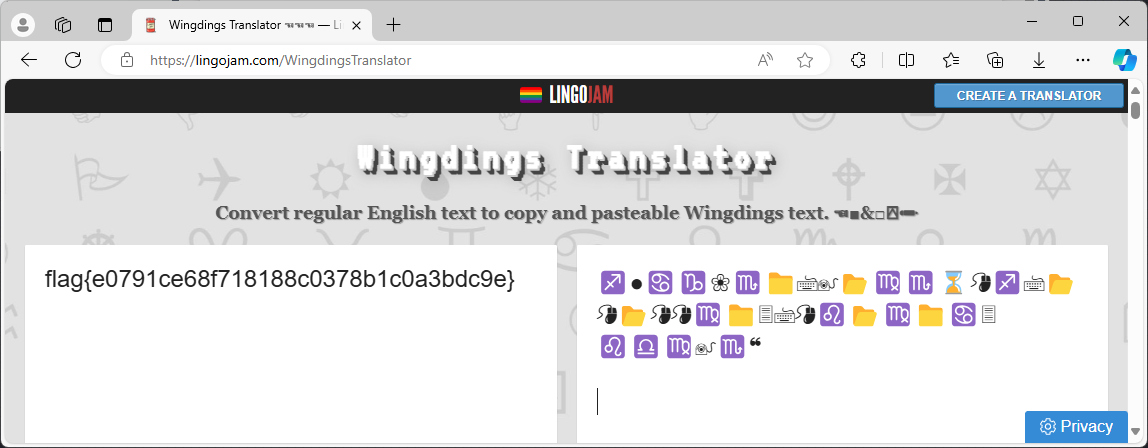
\includegraphics[width=16cm]{chicken-wings/screnshot.png}
\end{center}

\noindent
The flag is \texttt{flag\{e0791ce68f718188c0378b1c0a3bdc9e\}}.
\subsection{Car keys}

The given string already looks like the flag, because of the \texttt{\{\}}-characters. That made me suspect it's some kind of simple cipher, and the other given word, \texttt{QWERTY}, is probably the key. I tried some different cipher tools online, focusing on the ones with a key. The one that worked is called the \textit{Keyed Ceasar Cipher}\footnote{https://www.boxentriq.com/code-breaking/keyed-caesar-cipher}. The result was \texttt{flag\{6f980c0101c8aa361977cac06508a3de\}}

\subsection{Esab64}

The challenge name is a hint on itself: reversing and base64 decoding are key to this challenge. Applying both to the given text, I'm not quite there yet, but then reversing again, I get the flag:

\begin{lstlisting} 
>>> import base64
>>> given_text = "mxWYntnZiVjMxEjY0kDOhZWZ4cjYxIGZwQmY2ATMxEzNlFjNl13X"
>>> given_text_reverse = given_text[::-1]
>>> given_text_reverse_decoded = base64.b64decode(given_text_reverse)
>>> given_text_reverse_decoded
b'_}e61e711106bd0db1b78efa894b1125bf{galf'
>>> given_text_reverse_decoded[::-1]
b'flag{fb5211b498afe87b1bd0db601117e16e}_'
\end{lstlisting}

\noindent
I don't know what that last underscore is doing there, but the flag is \texttt{flag\{fb5211b498afe87b1bd0db601117e16e\}}.

\subsection{Buzz}

Opening the given file in a hex editor, I see the first bytes are \texttt{1F 9D}. This is the magic number of \texttt{.z} files.

\begin{center}
    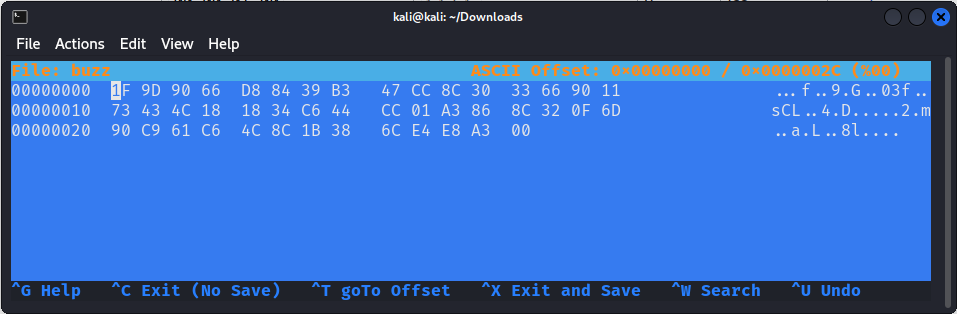
\includegraphics[width=16cm]{buzz/screenshot.png}
\end{center}

\noindent
After adding the right extension, I opened the file up in the default archive utility and found only one file inside, which contained the flag. The flag is \texttt{flag\{b3a33db7ba04c4c9052ea06d9ff17869\}}.

\section{Mobile}
\subsection{Andra}

I used apktool to decompile the given APK file, and then found the flag inside of an XML file:

\lstinputlisting[language=Bash]{andra/log.txt}

\noindent
The flag is visible in the result of this last \texttt{grep} call: \texttt{flag\{d9f72316dbe7ceab0db10bed1a738482\}}.

\subsection{Resourceful}

I used an online tool\footnote{https://apktool.org} to decompile the given APK, and had a look at the source code. The \texttt{MainActivity.java} file contains the password we'd need to access the app. 

\begin{center}
    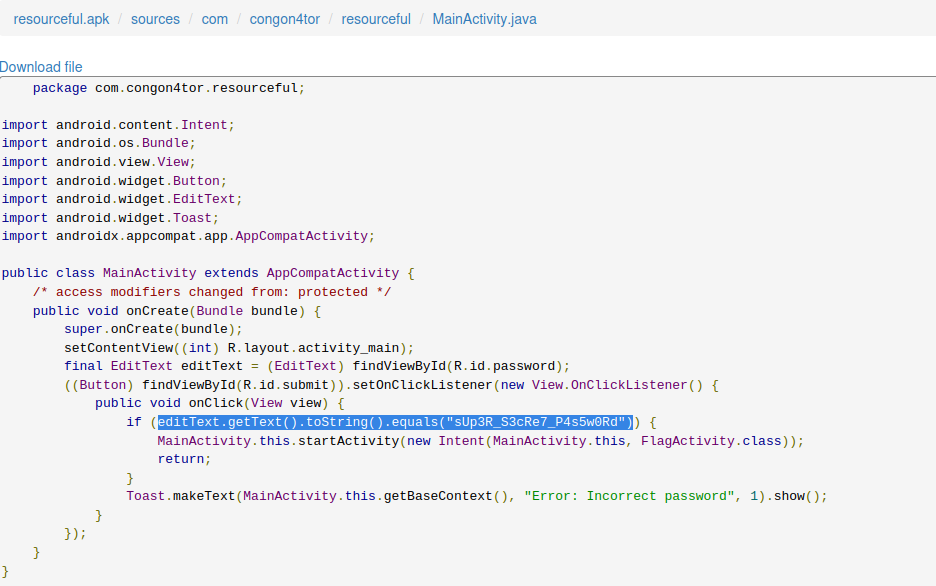
\includegraphics[width=16cm]{resourceful/screenshot1.png}
\end{center}

\noindent
I suppose I could install the app on a VM, use this password and I would maybe get the flag. However, the \texttt{startActivity} call below starts some \texttt{FlagActivity}. Inside, it looks like we are printing the flag:

\begin{center}
    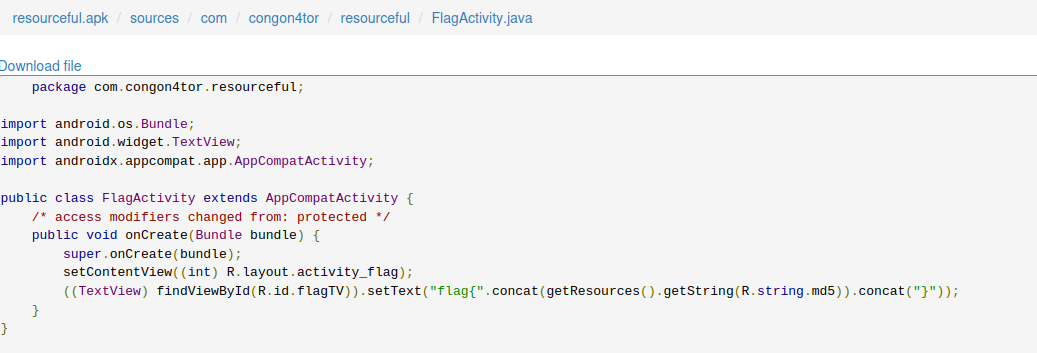
\includegraphics[width=16cm]{resourceful/screenshot2.png}
\end{center}

\noindent
The flag isn't in the code, however, it is stored in some resource called \texttt{md5} within \texttt{R}. I started looking for this value in the \texttt{resources} folder, and found two results:

\begin{center}
    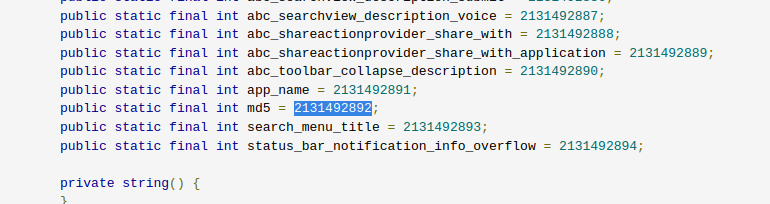
\includegraphics[width=16cm]{resourceful/screenshot3.png}
\end{center}

\begin{center}
    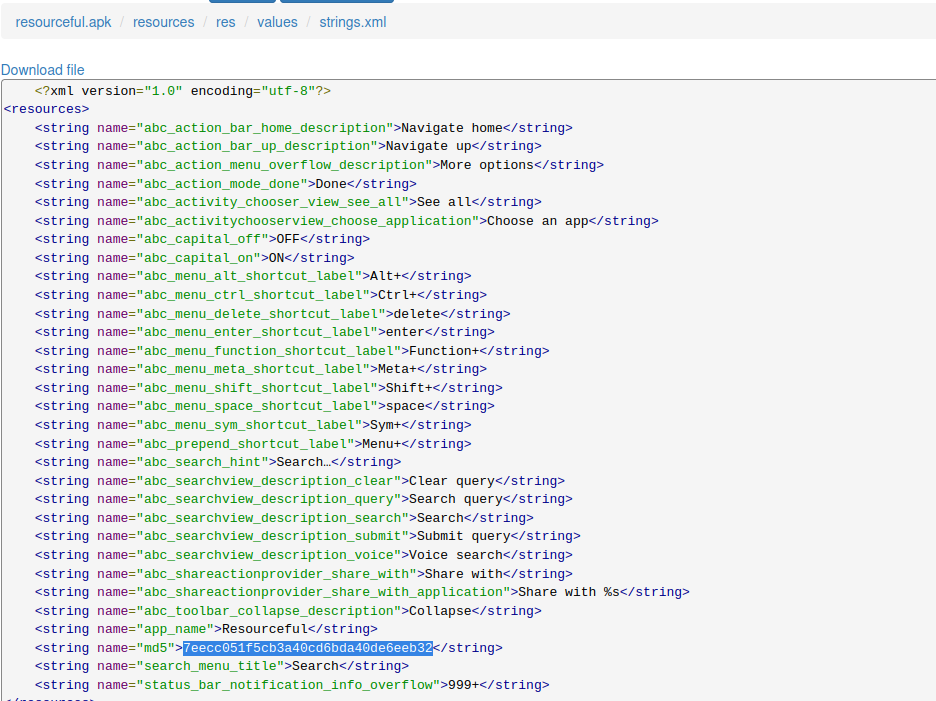
\includegraphics[width=16cm]{resourceful/screenshot4.png}
\end{center}

\noindent
The last one is the flag: \texttt{flag\{7eecc051f5cb3a40cd6bda40de6eeb32\}}.


\subsection{Microscopium}

Again, \texttt{apktool} was used to decompile the APK. Inside of the resulting files, I found something that looked a lot like compiled/minified JavaScript. That file is called \texttt{index.android.bundle}, which is a typical name for a \textit{React Native} bundle. I used the \textit{React Native Decompiler}\footnote{https://github.com/richardfuca/react-native-decompiler}, which threw out JavaScript that was a lot more readable, in separate module files. The \texttt{400.js} file contains the code that seems relevant: at least it handles the password/pin and decrypts something.

\begin{center}
    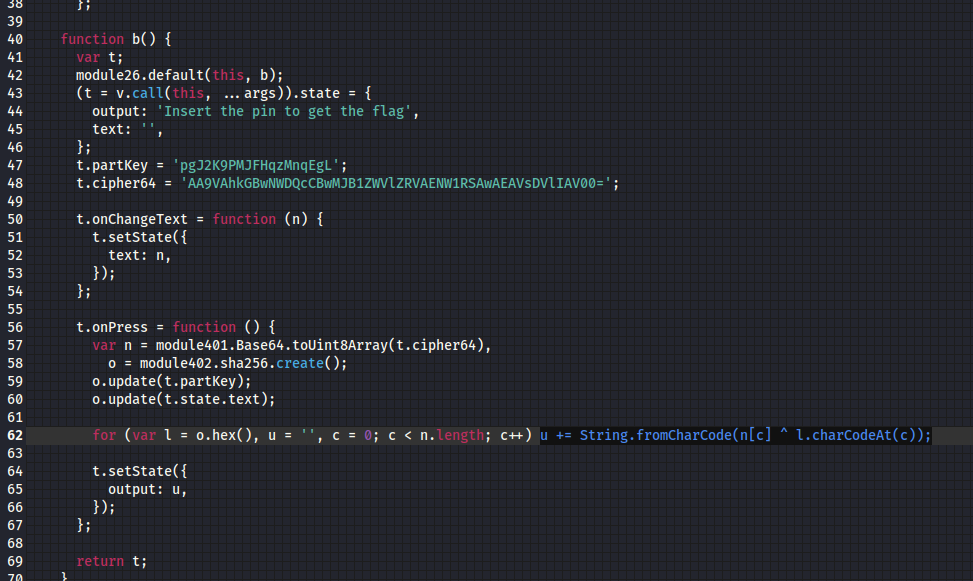
\includegraphics[width=16cm]{microscopium/screenshot.png}
\end{center}

\noindent
I recreated the relevant steps in this program in a separate JavaScript file, trying out different pin codes (assuming a 4-digit one first) using a loop. I couldn't get it to work with the actual module files, but from the context it was clear that those were \texttt{js-sha256} and \texttt{js-base64}, which I just pulled of NPM.


\lstinputlisting[language=Java]{microscopium/modified-script.js}

\noindent
Executing this, I got the flag: \texttt{flag\{06754e57e02b0c505149cd1055ba5e0b\}}


\section{Cryptography}
\subsection{Eaxy}

The name of this challenge immediately made me think of a XOR cipher. The \textit{XOR brute force} functionality in CyberChef, with \textit{"flag"} as known text, to the rescue:

\begin{center}
   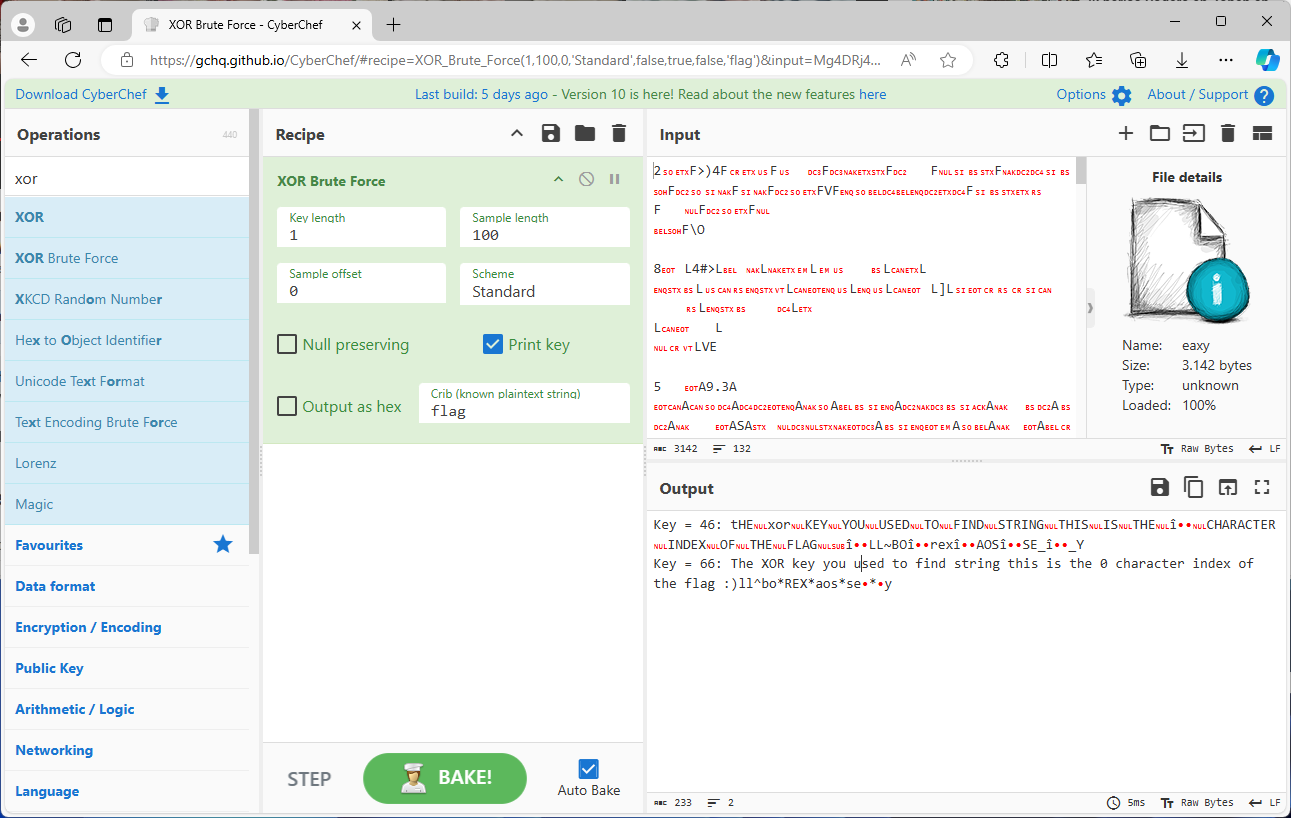
\includegraphics[width=\linewidth]{eaxy/screenshot.png}
\end{center}

\noindent
Assuming I can find every character of the string in a similar way, I wrote the following Python script to do exactly that.

\lstinputlisting[language=Python]{eaxy/solution.py}

\noindent
This got me the result \texttt{flag\{16edfce5c12443b61828af6cab90dc79\}}.



\end{document}
